%! TEX root = ../notes/main_notes.tex

\lecture{Hermit Economics}{lec-Hermit}

% Only appears in book/notes mode
\mode<article>{
	\section{Learning Objectives}
	\begin{itemize}
		\item Explain the meaning of opportunity cost.
		\item Demonstrate an understanding of the production function and the production possibilities frontier.
		\item Explain the role of diminishing marginal product.
	\end{itemize}
	
	\section{The Hermit}
	A hermit is someone who has chosen to live apart from society.  In the most extreme case, they have no contact with any other person and are completely self sufficient.  From a system thinking perspective, the hermit would be one element of the system, with the other elements being part of the ecological side of the hermit-nature social ecological system.
}

% Frame 1
\begin{frame}{Hermit System}
	\begin{itemize}
		\item Hermit,
		\begin{itemize}
			\item The social element of the social ecological system.
			\item Contributes labour and consumes the fruits of that labour.
		\end{itemize}
		\item Field,
		\begin{itemize}
			\item One ecological element of the system.
			\item Produces grain, with labour as the main input.
		\end{itemize}
		\item Lake.
		\begin{itemize}
			\item One ecological element of the system.
			\item Produces fish, with fishing effort (time spent fishing) as the main input.
		\end{itemize}
	\end{itemize}
\end{frame}

\mode<article>{
	The hermit can apply their time either to labour in the field, growing grain, or effort at the lake to catch fish.  The more labour applied in the field, the more grain that the hermit harvests.  Likewise, the more effort devoted to fishing, the more fish that will be caught.
		
}

\begin{frame}{Hermit System}
	\centering
	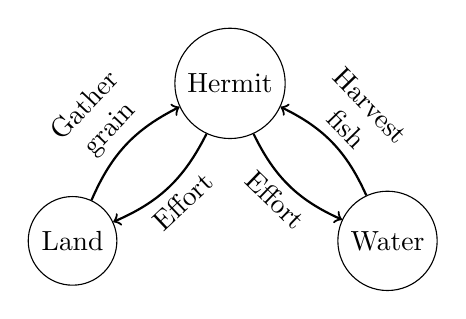
\begin{tikzpicture}
		% Define and place the nodes
		\node [circle, draw] at (3,3) (hermit) {Hermit};
		\node [circle, draw] at (1,1) (field) {Land};
		\node [circle, draw] at (5,1) (lake) {Water};
		
		% Draw edges
		\draw [->, thick] (hermit) to[bend left=20] node[below, sloped] {Effort} (field);
		\draw [->, thick] (field) to[bend left=20] node[above, sloped, align=center] {Gather \\ grain} (hermit);
		\draw [->, thick] (hermit) to[bend left=-20] node[below, sloped] {Effort} (lake);
		\draw [->, thick] (lake) to[bend left=-20] node[above, sloped, align=center] {Harvest \\ fish} (hermit);
		% \draw [->, thick] (field) to[bend right=20] node[above, sloped] {sediment} (lake);
	\end{tikzpicture}
\end{frame}

\begin{frame}{Human Ecology}
	\begin{columns}[T]
		\begin{column}{0.4\textwidth}
			\begin{itemize}
				\item Humans need food.
				\item Carbohydrates, fat and protein.
				\item Grain high in carbohydrates
				\item Fish provide fat and protein.
				\item Assume need fixed amounts of each.
			\end{itemize}
		\end{column}
		\begin{column}{0.6\textwidth}
			\centering
			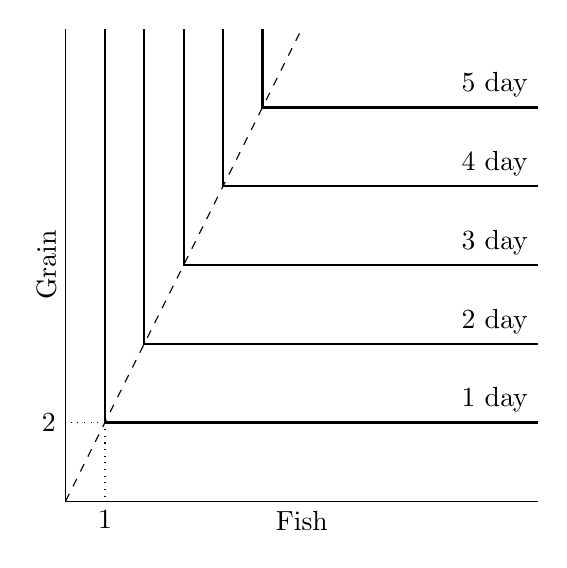
\begin{tikzpicture}
				\draw [-] (6,0) to node [below, sloped] {Fish} (0,0) to node [above, sloped] {Grain} (0,6) {};
				\draw [-, dashed] (0,0) to (3,6) {};
				\draw [-, thick] (6,1)  node [right, above left] {1 day} to (0.5,1) to (0.5,6);
				\draw [-, thick] (6,2)  node [right, above left] {2 day} to (1,2) to (1,6);
				\draw [-, thick] (6,3)  node [right, above left] {3 day} to (1.5,3) to (1.5,6);
				\draw [-, thick] (6,4)  node [right, above left] {4 day} to (2,4) to (2,6);
				\draw [-, thick] (6,5)  node [right, above left] {5 day} to (2.5,5) to (2.5,6);
				\draw [-, dotted] (0.5,1) to (0,1) node [left, left] {2};
				\draw [-, dotted] (0.5,1) to (0.5,0) node [below] {1};
			\end{tikzpicture}
		\end{column}
	\end{columns}
\end{frame}

\mode<article>{
	Humans need food to survive.  The basic components of that food are carbohydrates, fat and protein.  There are various specific nutrients and micronutrients we need.  So long as the fish and grain in our example provide sufficient quantities of these, we can focus on the balance of the three main nutrients.  For our model, we assume that the grain provides the carbohydrate requirements and the fish provide the fat and protein.
	
	One way to think about this is in terms of the number of days that a person has enough grain and fish to survive.  We can show this graphically using a contour map.  The dimensions of the map are the amount of fish and the amount of grain that the person has in their possesses.  Each contour line represents a day of survival.  
	
	The contours are 'L' shaped because survival for a day depends on consuming a minimum amount of each food source.  Consider the contour representing one day of survival.  The point where $q_F=1$ and $q_G=2$ is, in this example, the minimum amounts of fish and grain that are needed to survive one day.  If the person has more fish, but only the two units of grain, they will not survive more than one day.  Thus, with two units of grain, the contour for all larger quantities of fish always represents the same one day of survival.  
	
	The same logic applies when the person has one unit of fish.  For any amount of grain that is more than two, the person cannot survive any additional days.  Therefore the contour is vertical at the minimum amount of fish needed to survive one day.
	
	For the mathematically inclined, the function for the contours is
	
	\begin{equation}
		d(q_F,q_G) = \min\left(\frac{q_F}{\alpha_F},\frac{q_G}{\alpha_G}\right)
	\end{equation}
	
	In this equation, $\alpha_F$ and $\alpha_G$ are, respectively, the amounts of fish and grain that the person needs to consume per day to survive that day.  One can imagine that these amounts can differ by person.  One can also imagine that if there is a change in technology that translates fish and grain into nutrients could also change this relationship.  For example, a food preparation method that wastes less would reduce the amount needed per day of that food item.
	
	What have we not considered?  What would change if fish and grain decay?  The fact that the kinks in the figure follow a straight line, and the spacing of the contours is always the same assumes that there is no decay.  We know that grain can be stored far longer than raw fish.  If the fish is not processed into something that can be stored - dried for example - then how would the figure change?  What would happen if a share of the fish is lost each day?  What would happen if no fish can be consumed after it is five days old?
	
	Another thing to consider is that while grain has far more carbohydrates than it does have fat and protein, it does have some.  How would this change the graph?  In those cases, it will not have the tight kink.  Instead, it will have a bit of a curve, since there is some ability to substitute more grain for less fish.
}

\begin{frame}{Production Functions}
	\begin{itemize}
		\item A \emph{technology} is a way that inputs are converted to outputs.
		\item A \emph{production function} is a way of representing the technology.
		\begin{itemize}
			\item The production function is a simplification.
			\item The technology behaves the way that physics, chemistry, etc. require it to.
			\item All models are wrong, some are useful.
		\end{itemize}
		\item Three measures are commonly used to describe production at each input level.
		\begin{itemize}
			\item \emph{Total Product} is the total output produced given a particular input level.
			\item \emph{Average Product} is the total product divided by the input level.
			\item \emph{Marginal Product} is how much the total output changes if the level of input is changed by a small amount.
		\end{itemize}
	\end{itemize}
\end{frame}

\begin{frame}{The Fish Subsystem}
	\begin{itemize}
		\item Time path:
		\begin{enumerate}
			\item Travel from village to water
			\item Cast net
			\item Collect fish from net until can't carry any more
			\item Travel back to village
			\item Exchange fish for grain
		\end{enumerate}
		\item Each step of time path requires effort.
	\end{itemize}
\end{frame}

\mode<article>{
	If we consider the fish subsystem in relation to the village, we need to add a couple of elements that are not there when we just consider the relationship between effort and fish caught.  The fish harvester also needs to spend time traveling between the village and the water where fishing is done.
}
\begin{frame}{The Fish Subsystem}
	\centering
	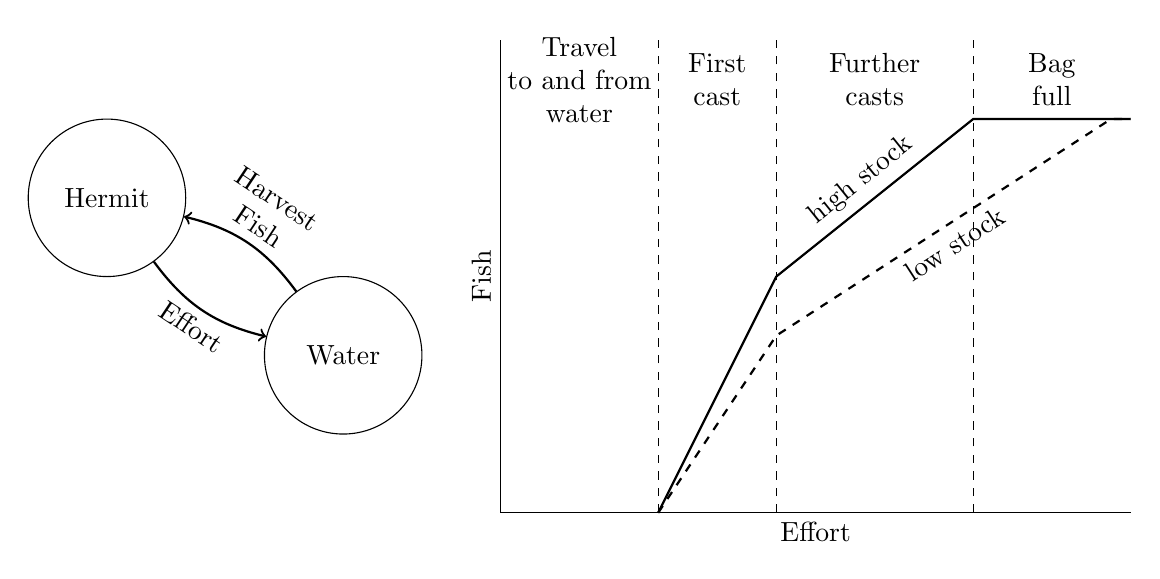
\begin{tikzpicture}
		% Define and place the nodes
		\node [circle, draw, minimum size=2cm, align=center] at (0,4) (fish) {Hermit};
		\node [circle, draw, minimum size=2cm, align=center] at (3,2) (water) {Water};
		
		% Draw edges
		\draw [->, thick, align=center] (water) to [bend right=20] node [above, sloped] {Harvest \\ Fish} (fish);
		\draw [->, thick, align=center] (fish) to [bend right=20] node [below, sloped] {Effort} (water);
		
		% Draw graph with production function
		\draw [-] (5,0) to node [above, sloped] {Fish} (5,6) {};
		\draw [-] (5,0) to node [below, sloped] {Effort} (13,0) {};
		\draw [-, thick] (7,0) to (8.5,3) to node [above, sloped] {high stock} (11,5) to (13,5) {};
		\draw [-, thick, dashed] (7,0) to (8.5,2.25) to node [below, sloped] {low stock} (12.75,5) to (13,5) {};
		\draw [-, dashed] (7,0) to (7,6) {};
		\draw [-, dashed] (8.5,0) to (8.5,6) {};
		\draw [-, dashed] (11,0) to (11,6) {};
		\node [align=center] at (6,5.5) {Travel \\ to and from \\ water};
		\node [align=center] at (7.75,5.5) {First \\ cast};
		\node [align=center] at (9.75,5.5) {Further \\ casts};
		\node [align=center] at (12,5.5) {Bag \\ full};
	\end{tikzpicture}
\end{frame}

\mode<artile>{
	The production function, if we start from the village and include travel time, a capacity constraint, and the reality of the fish movement, looks a bit more complicated.  
	
	There is an amount of effort needed to get to and from the water.  There are no fish produced until this amount of effort is provided.  
	
	The fish move around in the water.  It takes time for the fish to move.  When the fish harvester first arrives at the water, there are fish near where the harvester starts fishing from.  Thus, the first cast of the net captures a relatively large number of fish.  If the harvester says at the same location, then casting the net again will only catch fish that have moved into the area of the cast.  This means that further casts beyond the first will catch less fish.
	
	When the bag is full, then any extra effort does not add to the amount of fish that the fish harvester can bring back to the village.
	
	In the last chapter, we described the relationship between effort and harvest as dependent also on the size of the stock of fish in the water.  When we consider this stock effect, we would see the production function change shape.  For a lower stock, the first catch will catch less fish, as will the further casts.  Thus, it will take more effort to reach the capacity limit, where the harvester cannot bring any more fish back to the village.
}

\begin{frame}{The Grain Subsystem}
	\begin{itemize}
		\item Time path:
		\begin{enumerate}
			\item Travel from village to closest patch of land with grain.
			\item Harvest grain from patch.
			\item Move to next patch and repeat until grain bucket full.
			\item Travel back to village
			\item Exchange fish for grain
		\end{enumerate}
		\item Each step of time path requires effort.
	\end{itemize}
\end{frame}

\begin{frame}{The Grain Subsystem}
	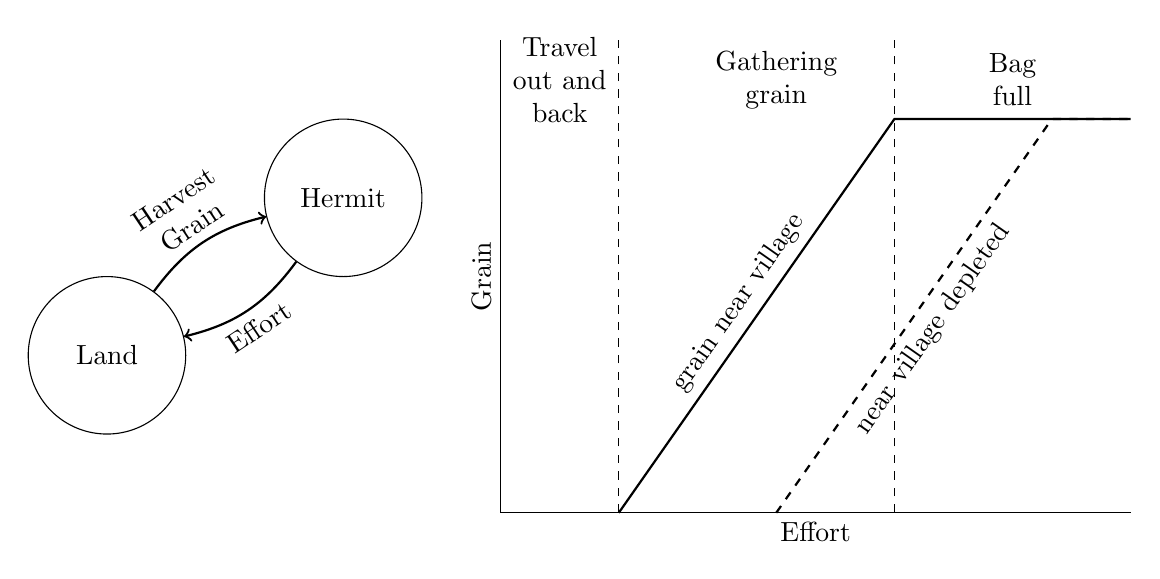
\begin{tikzpicture}
		% Define and place the nodes
		\node [circle, draw, minimum size=2cm, align=center] at (3,4) (gather) {Hermit};
		\node [circle, draw, minimum size=2cm, align=center] at (0,2) (land) {Land};
		
		% Draw edges
		\draw [->, thick, align=center] (land) to [bend left=20] node [above, sloped] {Harvest \\ Grain} (gather);
		\draw [->, thick, align=center] (gather) to [bend left=20] node [below, sloped] {Effort} (land);
		
		% Draw graph with production function
		\draw [-] (5,0) to node [above, sloped] {Grain} (5,6) {};
		\draw [-] (5,0) to node [below, sloped] {Effort} (13,0) {};
		\draw [-, thick] (6.5,0) to node [above, sloped] {grain near village} (10,5) to (13,5) {};
		\draw [-, thick, dashed] (8.5,0) to node [below, sloped] {near village depleted} (12,5) to (13,5) {};
		\draw [-, dashed] (6.5,0) to (6.5,6) {};
		\draw [-, dashed] (10,0) to (10,6) {};
		\node [align=center] at (5.75,5.5) {Travel \\ out and \\ back};
		\node [align=center] at (8.5,5.5) {Gathering \\ grain};
		\node [align=center] at (11.5,5.5) {Bag \\ full};
	\end{tikzpicture}
\end{frame}

\begin{frame}{Total, Average and Marginal Product}
	\begin{itemize}
		\item Total Product (TP) and Average Product (AP) are based on a level of input.
		\[
		AP = TP / E
		\]
		\begin{itemize}
			\item $E$ can be any input, not just effort.
		\end{itemize}
		\item Marginal Product (MP) is based on a small change in in the level of an input, around a specific level of that input.
		\[
		MP = \Delta TP / \Delta E = \partial TP / \partial E
		\]
		\begin{itemize}
			\item The marginal product measures how much extra output would be produced if a small amount of extra input is used.
			\item It is the slope of the production function at the input level.
			\item If production function is curved, slope of tangency line.
		\end{itemize}
	\end{itemize}
\end{frame}

\begin{frame}{The Fish Subsystem}
	\centering
	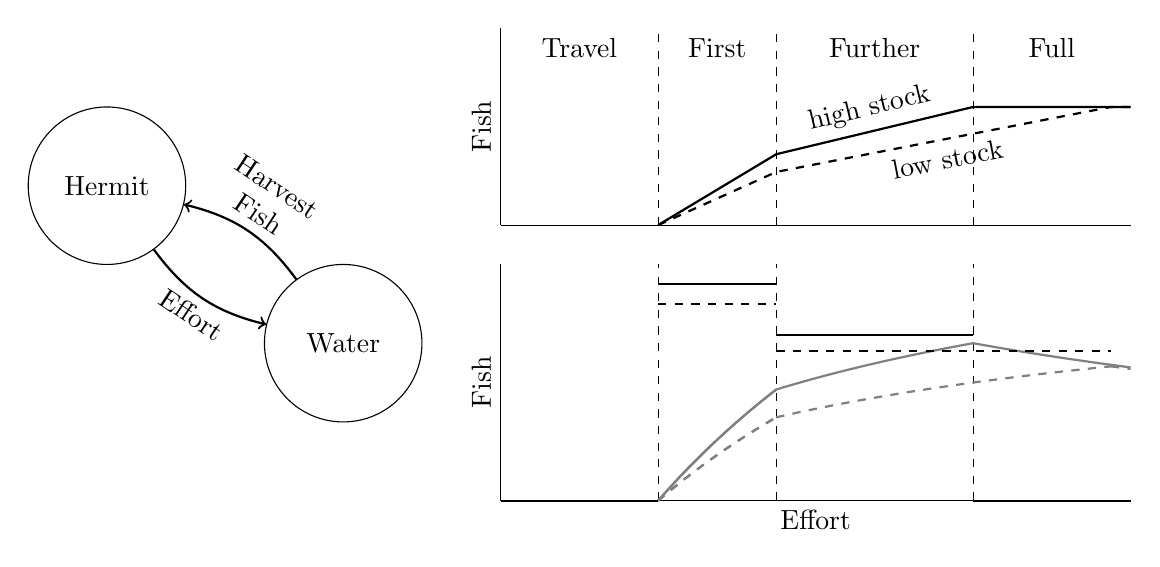
\begin{tikzpicture}
		% Define and place the nodes
		\node [circle, draw, minimum size=2cm, align=center] at (0,4) (fish) {Hermit};
		\node [circle, draw, minimum size=2cm, align=center] at (3,2) (water) {Water};
		
		% Draw edges
		\draw [->, thick, align=center] (water) to [bend right=20] node [above, sloped] {Harvest \\ Fish} (fish);
		\draw [->, thick, align=center] (fish) to [bend right=20] node [below, sloped] {Effort} (water);
		
		% Draw graph with production function in top panel
		\draw [-] (5,3.5) to node [above, sloped] {Fish} (5,6) {};
		\draw [-] (5,3.5) to node [below, sloped] {} (13,3.5) {};
		\draw [-, thick] (7,3.5) to (8.5,4.4) to node [above, sloped] {high stock} (11,5) to (13,5) {};
		\draw [-, thick, dashed] (7,3.5) to (8.5,4.175) to node [below, sloped] {low stock} (12.75,5) to (13,5) {};
		\draw [-, dashed] (7,3.5) to (7,6) {};
		\draw [-, dashed] (8.5,3.5) to (8.5,6) {};
		\draw [-, dashed] (11,3.5) to (11,6) {};
		\node [align=center] at (6,5.75) {Travel};
		\node [align=center] at (7.75,5.75) {First};
		\node [align=center] at (9.75,5.75) {Further};
		\node [align=center] at (12,5.75) {Full};
		
		% draw lower panel with marginal and average product
		\draw [-] (5,0) to node [above, sloped] {Fish} (5,3) {};
		\draw [-] (5,0) to node [below, sloped] {Effort} (13,0) {};
		\draw [-, dashed] (7,0) to (7,3) {};
		\draw [-, dashed] (8.5,0) to (8.5,3) {};
		\draw [-, dashed] (11,0) to (11,3) {};
		
		% plot the average product
		\draw [-,thick,gray] (5,0) to (7,0) {};
		\draw [thick,gray,domain=7:8.5,samples=30] plot (\x, {8 * (\x - 7) / \x});
		\draw [thick,gray,domain=7:8.5,samples=30] plot (\x, {8 * (\x - 7) / \x});
		\draw [thick,gray,domain=8.5:11,samples=30] plot (\x, {(1.5 * 8 + 4 * (\x - 8.5)) / \x});
		\draw [thick,gray,domain=11:13,samples=30] plot (\x, {(1.5 * 8 + 4 * 2.5) / \x});
		\draw [-,thick,gray,dashed] (5,0) to (7,0) {};
		\draw [thick,gray,dashed,domain=7:8.5,samples=30] plot (\x, {6 * (\x - 7) / \x});
		\draw [thick,gray,dashed,domain=7:8.5,samples=30] plot (\x, {6 * (\x - 7) / \x});
		\draw [thick,gray,dashed,domain=8.5:12.75,samples=30] plot (\x, {(1.5 * 6 + 3 * (\x - 8.5)) / \x});
		\draw [thick,gray,dashed,domain=12.75:13,samples=30] plot (\x, {(1.5 * 6 + 3 * 4.25) / \x});
		
		% plot the marginal product
		\draw [-,thick] (5,0) to (7,0) {};
		\draw [-,thick] (7,2.75) to (8.5,2.75) {};
		\draw [-,thick] (8.5,2.1) to (11,2.1) {};
		\draw [-,thick] (11,0) to (13,0) {};
		\draw [-,thick,dashed] (5,0) to (7,0) {};
		\draw [-,thick,dashed] (7,2.5) to (8.5,2.5) {};
		\draw [-,thick,dashed] (8.5,1.9) to (12.75,1.9) {};
		\draw [-,thick,dashed] (12.75,0) to (13,0) {};
	\end{tikzpicture}
\end{frame}

\mode<article>{
	The average product for the fish production function is zero until the level of effort is reached where the effort is sufficient for travel to and from the hermit's home.  After this point it climbs, at a slowly decreasing rate.  The curvature is subtle in the graph, but it is there.  Once the first net cast is hauled in, the later casts catch less fish.  The rate of increase of the average product slows.  Once the fish basket is full, there are no further fish caught.  From this level, the average product is downward sloping, with the slope becoming less steep as effort continues to increase.
	
	The marginal product is also zero until the first net cast.  Through the first net cast, it is at its highest.  When fish are being pulled into the basked from the second cast, the extra fish per unit of effort is lower.  Once the basket is full, extra effort does not add any more fish to the basket, so the marginal product is again zero.
	
	Notice that when the average product is increasing, the marginal product is above the average product, and when the marginal product is decreasing, it is below the average product.  This is a general result.
}

\begin{frame}{The Grain Subsystem}
	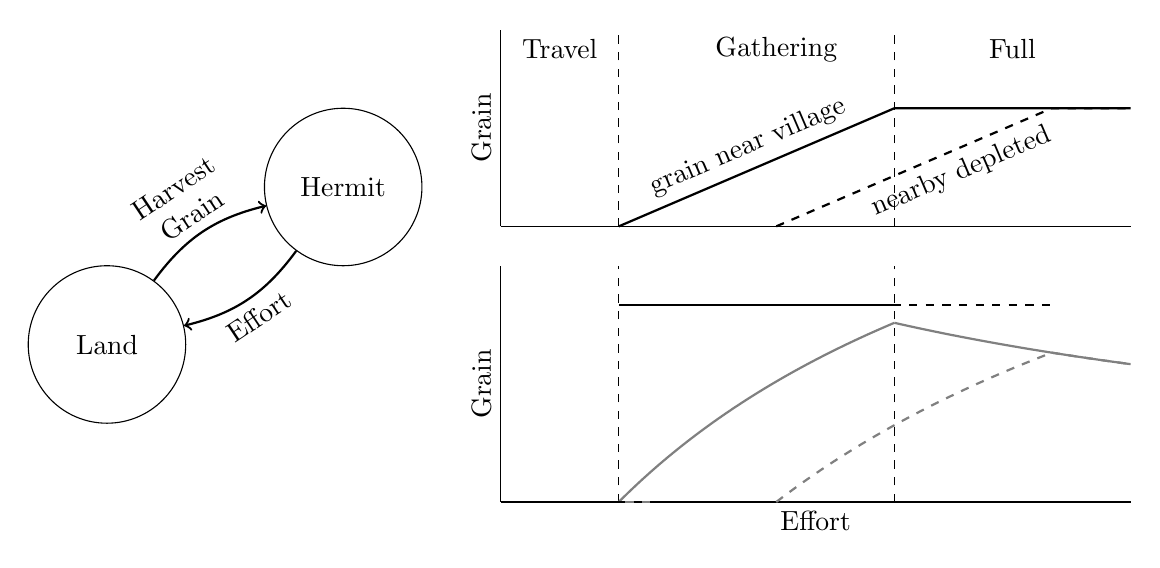
\begin{tikzpicture}
		% Define and place the nodes
		\node [circle, draw, minimum size=2cm, align=center] at (3,4) (gather) {Hermit};
		\node [circle, draw, minimum size=2cm, align=center] at (0,2) (land) {Land};
		
		% Draw edges
		\draw [->, thick, align=center] (land) to [bend left=20] node [above, sloped] {Harvest \\ Grain} (gather);
		\draw [->, thick, align=center] (gather) to [bend left=20] node [below, sloped] {Effort} (land);
		
		% Draw graph with production function
		\draw [-] (5,3.5) to node [above, sloped] {Grain} (5,6) {};
		\draw [-] (5,3.5) to node [below, sloped] {} (13,3.5) {};
		\draw [-, thick] (6.5,3.5) to node [above, sloped] {grain near village} (10,5) to (13,5) {};
		\draw [-, thick, dashed] (8.5,3.5) to node [below, sloped,xshift=15pt] {nearby depleted} (12,5) to (13,5) {};
		\draw [-, dashed] (6.5,3.5) to (6.5,6) {};
		\draw [-, dashed] (10,3.5) to (10,6) {};
		\node [align=center] at (5.75,5.75) {Travel};
		\node [align=center] at (8.5,5.75) {Gathering};
		\node [align=center] at (11.5,5.75) {Full};

		% draw lower panel with marginal and average product
		\draw [-] (5,0) to node [above, sloped] {Grain} (5,3) {};
		\draw [-] (5,0) to node [below, sloped] {Effort} (13,0) {};
		\draw [-, dashed] (6.5,0) to (6.5,3) {};
		\draw [-, dashed] (10,0) to (10,3) {};
		
		% plot the average product
		\draw [-,thick,gray] (5,0) to (7,0) {};
		\draw [thick,gray,domain=6.5:10,samples=100] plot (\x, {6.5 * (\x - 6.5) / \x});
		% \draw [thick,gray,domain=7:8.5,samples=30] plot (\x, {8 * (\x - 7) / \x});
		\draw [thick,gray,domain=10:13,samples=30] plot (\x, {(3.5 * 6.5) / \x});
		% \draw [thick,gray,domain=11:13,samples=30] plot (\x, {(1.5 * 8 + 4 * 2.5) / \x});
		\draw [-,thick,gray,dashed] (5,0) to (7,0) {};
		\draw [thick,gray,dashed,domain=8.5:12,samples=30] plot (\x, {6.5 * (\x - 8.5) / \x});
		% \draw [thick,gray,dashed,domain=7:8.5,samples=30] plot (\x, {6 * (\x - 7) / \x});
		% \draw [thick,gray,dashed,domain=8.5:12.75,samples=30] plot (\x, {(1.5 * 6 + 3 * (\x - 8.5)) / \x});
		\draw [thick,gray,dashed,domain=12:13,samples=30] plot (\x, {(3.5 * 6.5) / \x});
		
		% plot the marginal product
		\draw [-,thick] (5,0) to (6.5,0) {};
		\draw [-,thick] (6.5,2.5) to (10,2.5) {};
		\draw [-,thick] (10,0) to (13,0) {};
		\draw [-,thick,dashed] (5,0) to (8.5,0) {};
		\draw [-,thick,dashed] (8.5,2.5) to (12,2.5) {};
		\draw [-,thick,dashed] (12,0) to (13,0) {};
	\end{tikzpicture}
\end{frame}

\mode<article>{
	The average and marginal product curves for the grain gathering are similar to those for the fish harvesting.  In both cases, the marginal and average product are both zero until the travel requirements are satisfied.  After that, the average product increases until the bucket is full.  Since the slope of the production function is constant, the marginal product is also constant.  Notice that with the difference between the two production functions being only the effort needed to get to and then back from the patches with grain, depleting the patches near the village does not change the marginal product.  It does lower the average product, since the total effort needed for any amount of grain gathered is higher.
}

\mode<article>{
	Our hermit can divide their effort between gathering grain or harvesting fish (or staying at home and resting).  We can plot these combinations of fish and grain in what in economics is call a \textbf{\textit{production possibilities frontier (PPF)}}.  It is a frontier because it is what could be produced if all effort is used.  In the figure, the combination marked $E_1$ is the amount of production of fish and grain that can occur if there is only enough effort available to travel between the harvest and gathering sites and the hermit's home.
	
	If the hermit has sufficient food to allow them to survive beyond the travel time, then we can examine the combinations of fish and grain that the hermit can produce by dividing their effort in different ways between fishing and gathering.  For the curves represented by $E_2$ and $E_3$, if the effort is reallocated from harvesting fish to gathering grain, the amount of fish harvested decreases and the amount of grain harvested increases.
	
	With the PPF labeled $E_4$, the limit of what the fish basket can hold has been reached.  In effect, the hermit 'throws away' part of the total effort, as it is dedicating it to catching fish, which cannot be take back home.  Since the first cast is the most productive, the hermit is in fact throwing away the most productive effort when running up against this constraint.  If this seems strange, think of the order of events.  The hermit cannot devote effort to later catches until they have made the first cast.
	
	The PPF labeled $E_5$ corresponds to an effort level where one of the grain bucket or fish basket is full for most of the effort divisions.  There is in effect a lot of wasted effort here, as it is being applied to activities which cannot result in any more grain or fish being brought back home.  We might think of this wasted effort as leisure.  If the hermit has enough food to sustain themselves for this many days, maybe it would be better for them to stay at home, enjoying themselves while eating the stockpiled food, heading out when they have enough food left to fill their basket or bucket and bring it back home.
}

\begin{frame}{Production Possibilities}
	\begin{columns}[T]
		\begin{column}{0.3\textwidth}
			\begin{itemize}
				\item Split total effort between fish and grain.
				\item $E_5 > E_4 > E_3 > E_2 > E_1$
				\item At $E_1$, no fish caught or grain gathered.
				\item At $E_5$, most effort not used, as bucket or basket full.
			\end{itemize}
		\end{column}
		\begin{column}{0.7\textwidth}
			\centering
			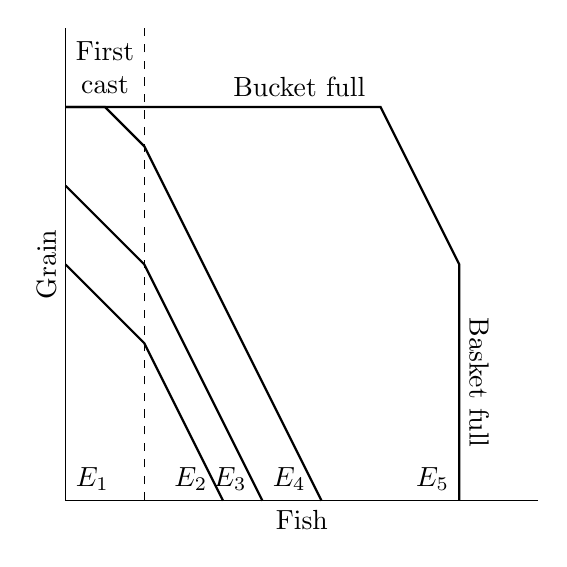
\begin{tikzpicture}
				% Axes for plot
				\draw [-] (6,0) to node [below, sloped] {Fish} (0,0) to node [above, sloped] {Grain} (0,6);
				% \draw [-,thick] (3,0) to (2,1) to (0,2) node [left, right, yshift=2pt] {$E_2$};
				% \draw [-,thick] (4,0) to (3,1) to (0,2.5) node [left, right, yshift=2pt] {$E_3$};
				% \draw [-,thick] (5,0) to (5,0.5) to (4.5,1) to (0,3.25) node [left, right, yshift=2pt] {$E_4$};
				\draw [-,thick] (0,3) to (1,2) to (2,0) node [above left, xshift=-2pt] {$E_2$};
				\draw [-,thick] (0,4) to (1,3) to (2.5,0) node [above left, xshift=-2pt] {$E_3$};
				\draw [-,thick] (0,5) to (0.5,5) to (1,4.5) to (3.25,0) node [above left, xshift=-2pt] {$E_4$};
				\draw [-,thick] (0,5) to node [above right, sloped] {Bucket full} (4,5) to (5,3) to 
				node [right, above, sloped] {Basket full}(5,0) node [left, above left] {$E_5$};
				\draw [-,dashed] (1,0) to (1,6) {};
				\draw [-,thick] (0,0) node [above right] {$E_1$} to (0,0) {};
				\node [align=center] at (0.5,5.5) {First \\ cast};
			\end{tikzpicture}
		\end{column}
	\end{columns}
\end{frame}

\mode<article>{
	The PPF maps the different combinations of fish and grain that can be produced for a particular level of effort.  It shows the impact of reallocating effort from the production of fish to the production of grain.  Moving between points along the PPF involves reducing the amount of one good produced and increasing the amount of the other produced.
	
	\textbf{\textit{Opportunity cost}} is defined as \textit{the value of the next best alternative foregone}.  The production possibilities frontier is one way to illustrate opportunity cost.  In the figure, three changes in the amount of grain are produced, for the PPF that was labeled $E_4$ in the previous figure. 
	
	If fish production is increased by $\Delta F_1$, there is no reduction in grain production.  For this change in fish, the grain bucket is full and the effort beyond filling the grain bucket is not adding anything to the bucket.  In this situation, moving effort to harvesting fish has no impact on the grain gathered.  The opportunity cost of this increase in fish harvested is zero grain gathered.
	
	For the increase in fish represented by $\Delta F_2$, the amount of grain harvested falls by $\Delta G_2$.  The effort being applied to fishing here is part of the first cast, when the effort is most effective.  When more effort is put to fish harvesting, adding $\Delta F_3$, we have moved into the further casts, where less fish have had time to move into the area where the net is cast, and therefore less fish are collected for the same amount of effort.  Therefore, there is now a larger amount of effort taken away from gathering grain to realize the increased fish harvest.
	
	This is a result we expect to be generally true.  As we take more resources away from producing one good, in this case grain, the resource that we are taking away is more productive.  With the production function, we saw that the marginal product decreased as effort increased.  As we add more effort, the contribution of an extra unit of effort to total production falls.  If we are moving effort from one good to another, the good that we are taking effort away from is moving to a higher marginal product part of the production function, while for the good that is getting more effort, we are moving to a lower marginal product part of the production function.  Taken together, as we move from high grain production and low fish production to high fish production and low grain production, the amount of grain we give up to get an extra unit of fish increases.
}

\begin{frame}{Opportunity Cost}
	\begin{columns}[T]
		\begin{column}{0.3\textwidth}
			\begin{itemize}
				\item Increase fish by $\Delta F_1$ for no reduction in grain.
				\item Increase fish by $\Delta F_2$ for reduction in grain of $\Delta G_2$.
				\item Increase fish by $\Delta F_3$ for reduction in grain of $\Delta G_3$.
			\end{itemize}
		\end{column}
		\begin{column}{0.7\textwidth}
			\centering
			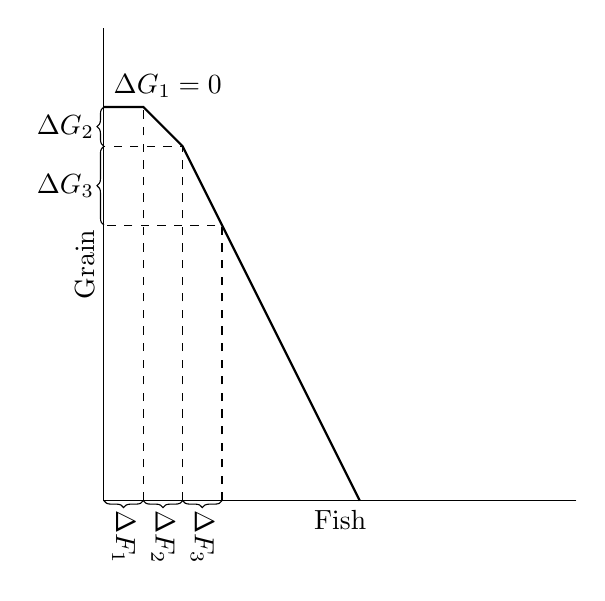
\begin{tikzpicture}
				% Axes for plot
				\draw [-] (6,0) to node [below, sloped] {Fish} (0,0) to node [above, sloped] {Grain} (0,6);
				% \draw [-,thick] (3,0) to (2,1) to (0,2) node [left, right, yshift=2pt] {$E_2$};
				% \draw [-,thick] (4,0) to (3,1) to (0,2.5) node [left, right, yshift=2pt] {$E_3$};
				\draw [-,thick] (0,5) to (0.5,5) to (1,4.5) to (3.25,0) {};
				% \draw [-,thick] (5,0) to node [above right, sloped] {Basket full} (5,4) to (3,5) to 
				% node [right, above, sloped] {Bucket full}(0,5) node [left, below right] {$E_5$};
				\draw [-,dashed] (1.5,0) to (1.5,3.5) to (0,3.5) {};
				\draw [-,dashed] (1,0) to (1,4.5) to (0,4.5) {};
				\draw [-,dashed] (0.5,0) to (0.5,5) {};
				\node [right, rotate=-90] at (0.25,0) {$\Delta F_1$};
				\draw [decorate, decoration={brace,mirror}] (0,0) to (0.5,0);
				\node [right, rotate=-90] at (0.75,0) {$\Delta F_2$};
				\draw [decorate, decoration={brace,mirror}] (0.5,0) to (1,0);
				\node [right, rotate=-90] at (1.25,0) {$\Delta F_3$};
				\draw [decorate, decoration={brace,mirror}] (1,0) to (1.5,0);
				\node [left] at (0,4) {$\Delta G_3$};
				\draw [decorate, decoration={brace}] (0,3.5) to (0,4.5);
				\node [left] at (0,4.75) {$\Delta G_2$};
				\draw [decorate, decoration={brace}] (0,4.5) to (0,5);
				\node [above right] at (0,5) {$\Delta G_1 = 0$};
				% \draw [-,thick] (0,0) node [above right] {$E_1$} to (0,0) {};
				% \node [align=center] at (5.5,0.5) {First \\ cast};
			\end{tikzpicture}
		\end{column}
	\end{columns}
\end{frame}

\mode<article>{
	When the production functions were described above, some aspects relevant to sustainability were illustrate that do not show up here.  For fishing, if harvesting reduces the fish stock, then the production function slope becomes flatter.  It will take more effort, more days spent fishing, to fill up the fish basket.  This shows up in the PPF as a rotation inward around the intercept with the Grain axis.  The decline in the fish stock does not affect the amount of grain that can be gathered, if all the effort is devoted to gathering grain.  However, the amount of grain production that is given up to harvest another fish increases.
	
	When the grain available in patches near the village is depleted, more effort must be spent on travel.  This reduces the total effort available for both activities, if we start from the same premise where we only examine how to reallocate effort after enough food is devoted to enabling both the fish harvester and the grain gatherer to travel to and from their respective activity locations.  The PPF shifts left, lowering the intersection with the Grain axis.  Since the total effort to divide is reduced, there is no longer enough effort to fill the fish basket, even when all the effort is put toward fishing.
}

\begin{frame}{Production Possibilities}
	\centering
	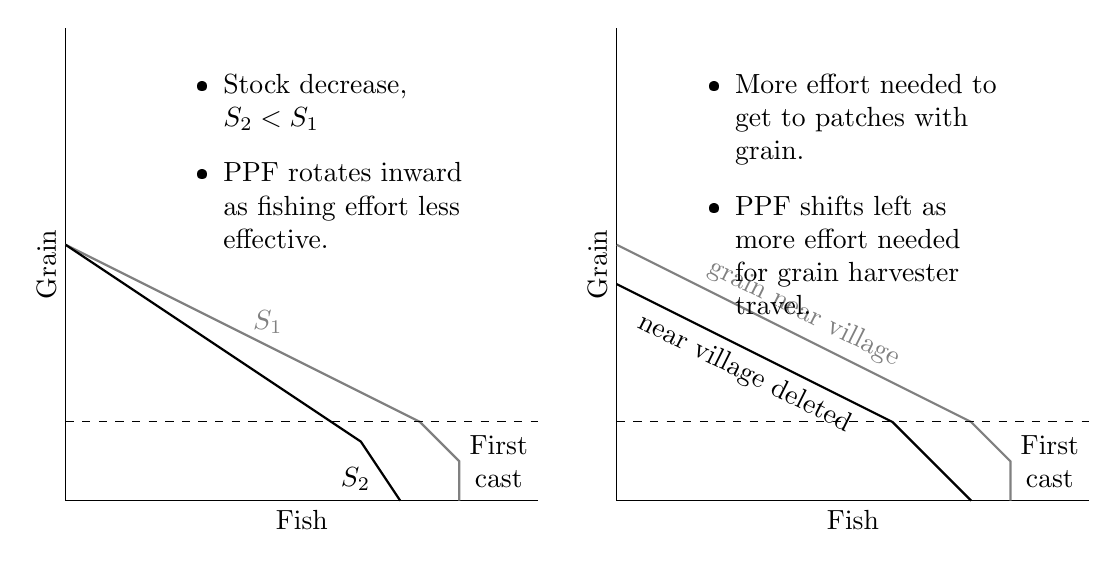
\begin{tikzpicture}
		\coordinate (ListBase) at (6.5,6);
		% Left figure
		\draw [-] (6,0) to node [below, sloped] {Fish} (0,0) to node [above, sloped] {Grain} (0,6);
		\draw [-,thick,gray] (5,0) to (5,0.5) to (4.5,1) to node [left, right, yshift=4pt] {$S_1$} (0,3.25) {};
		\draw [-,thick] (4.25,0) to node [left, below left, yshift=5pt] {$S_2$} (3.75,0.75) to (0,3.25) {};
		\draw [-,dashed] (0,1) to (6,1) {};
		\node [align=center] at (5.5,0.5) {First \\ cast};
		\node [anchor=north west, text width=0.35\textwidth] at ([xshift=-5.5cm]ListBase) {
			\begin{itemize}
				\item Stock decrease, $S_2 < S_1$
				\item PPF rotates inward as fishing effort less effective.
			\end{itemize}
		};
		% Right figure, more travel for grain harvest
		\draw [-] (13,0) to node [below, sloped] {Fish} (7,0) to node [above, sloped] {Grain} (7,6);
		\draw [-,thick,gray] (12,0) to (12,0.5) to (11.5,1) to node [above, sloped] {grain near village} (7,3.25) {};
		\draw [-,thick] (11.5,0) to (10.5,1) to node [below, sloped] {near village deleted} (7,2.75) {};
		\draw [-,dashed] (7,1) to (13,1) {};
		\node [align=center] at (12.5,0.5) {First \\ cast};
		\node [anchor=north west, text width=0.35\textwidth] at ([xshift=1cm]ListBase) {
			\begin{itemize}
				\item More effort needed to get to patches with grain.
				\item PPF shifts left as more effort needed for grain harvester travel.
			\end{itemize}
		};
		
	\end{tikzpicture}
\end{frame}

\mode<article>{
	The production possibilities frontier tells us what combinations of fish and grain can be produced by the villagers, for different levels of effort.  The biological reality of our villagers requires that the consume a particular bundle of fish and grain each day.  If we put the biology together with the production possibilities frontier, we can see how to allocate the effort to provide the most days of life for the villagers.
}

\begin{frame}{Production Possibilities}
	\begin{columns}[T]
		\begin{column}{0.3\textwidth}
			\begin{itemize}
				\item Lifespans $L_1$ and $L_2$ are attainable.
				\begin{itemize}
					\item At \textbf{b} attain $L_1$.
					\item At \textbf{a} attain $L_2$.
					\item Same effort level.
				\end{itemize}
				\item Lifespans $L_3$, $L_4$ and $L_5$ are not attainable.
			\end{itemize}
		\end{column}
		\begin{column}{0.7\textwidth}
			\centering
			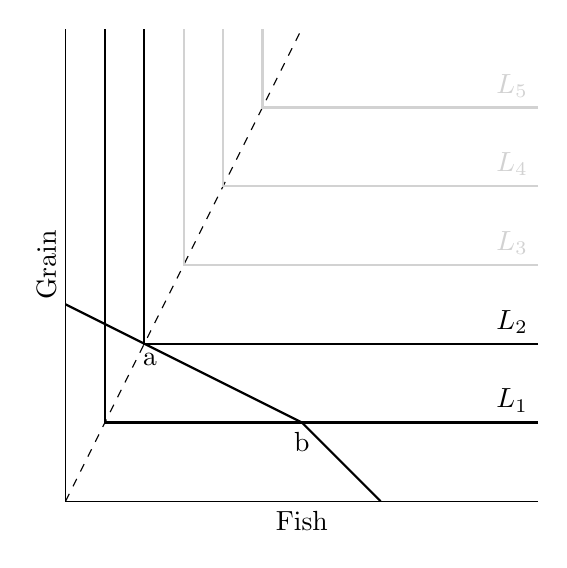
\begin{tikzpicture}
				% Axes for plot
				\draw [-] (6,0) to node [below, sloped] {Fish} (0,0) to node [above, sloped] {Grain} (0,6);
				% \draw [-,thick] (3,0) to (2,1) to (0,2) node [left, right, yshift=2pt] {$E_2$};
				\draw [-,thick] (4,0) to (3,1) to (0,2.5) node [left, right, yshift=2pt] {};
				% \draw [-,thick] (5,0) to (5,0.5) to (4.5,1) to (0,3.25) node [left, right, yshift=2pt] {$E_4$};
				% \draw [-,thick] (5,0) to node [above right, sloped] {Basket full} (5,4) to (3,5) to 
				% node [right, above, sloped] {Bucket full}(0,5) node [left, below right] {$E_5$};
				% \draw [-,dashed] (0,1) to (6,1) {};
				% \draw [-,thick] (0,0) node [above right] {$E_1$} to (0,0) {};
				% \node [align=center] at (5.5,0.5) {First \\ cast};
				
				% Indifference curves
				\draw [-, dashed] (0,0) to (3,6) {};
				\draw [-, thick] (6,1) node [right, above left] {$L_1$} to (0.5,1) to (0.5,6);
				\draw [-, thick] (6,2) node [right, above left] {$L_2$} to (1,2) to (1,6);
				\draw [-, thick, gray!35] (6,3) node [right, above left] {$L_3$} to (1.5,3) to (1.5,6);
				\draw [-, thick, gray!35] (6,4) node [right, above left] {$L_4$} to (2,4) to (2,6);
				\draw [-, thick, gray!35] (6,5) node [right, above left] {$L_5$} to (2.5,5) to (2.5,6);
				\node [below, xshift=2pt] at (1,2) {a}; 
				\node [below] at (3,1) {b};
			\end{tikzpicture}
		\end{column}
	\end{columns}
\end{frame}

\mode<article>{
	Putting together the human needs and the production possibilities lets us identify something we might see as optimal.  It seems reasonable to think that dividing up the resources that the villagers have in such a way as to maximize the number of days that they continue living would be a reasonable objective.
	
	Can we expect this outcome from people who interact independently?  
}
